\documentclass[conference]{IEEEtran}
\IEEEoverridecommandlockouts
% The preceding line is only needed to identify funding in the first footnote. If that is unneeded, please comment it out.
\usepackage{cite}
\usepackage{amsmath,amssymb,amsfonts}
\usepackage{algorithmic}
\usepackage{graphicx}
\usepackage{textcomp}
\usepackage{xcolor}
\def\BibTeX{{\rm B\kern-.05em{\sc i\kern-.025em b}\kern-.08em
    T\kern-.1667em\lower.7ex\hbox{E}\kern-.125emX}}

\ifCLASSINFOpdf
\else
    \usepackage[dvips]{graphicx}
\fi
\usepackage{url}
\usepackage{listings}
% \usepackage[margin=1in]{geometry}
\usepackage{amsmath,amsthm,amssymb}
\usepackage{amsmath,amsthm,amssymb}
\usepackage[spanish]{babel} %Castellanización
\usepackage[T1]{fontenc} %escribe lo del teclado
\usepackage[utf8]{inputenc} %Reconoce algunos símbolos
\usepackage{lmodern} %optimiza algunas fuentes
\usepackage{blkarray}
\graphicspath{ {images/} }
\usepackage{hyperref} % Uso de links

\newcommand{\N}{\mathbb{N}}
\newcommand{\Z}{\mathbb{Z}}
\usepackage{float}
\newenvironment{theorem}[2][Theorem]{\begin{trivlist}
\item[\hskip \labelsep {\bfseries #1}\hskip \labelsep {\bfseries #2.}]}{\end{trivlist}}
\newenvironment{lemma}[2][Lemma]{\begin{trivlist}
\item[\hskip \labelsep {\bfseries #1}\hskip \labelsep {\bfseries #2.}]}{\end{trivlist}}
\newenvironment{exercise}[2][Exercise]{\begin{trivlist}
\item[\hskip \labelsep {\bfseries #1}\hskip \labelsep {\bfseries #2.}]}{\end{trivlist}}
\newenvironment{problem}[2][Problem]{\begin{trivlist}
\item[\hskip \labelsep {\bfseries #1}\hskip \labelsep {\bfseries #2.}]}{\end{trivlist}}
\newenvironment{question}[2][Question]{\begin{trivlist}
\item[\hskip \labelsep {\bfseries #1}\hskip \labelsep {\bfseries #2.}]}{\end{trivlist}}
\newenvironment{corollary}[2][Corollary]{\begin{trivlist}
\item[\hskip \labelsep {\bfseries #1}\hskip \labelsep {\bfseries #2.}]}{\end{trivlist}}
\newcommand*{\defeq}{\stackrel{\text{def}}{=}}
\newenvironment{solution}{\begin{proof}[Solution]}{\end{proof}}
\hyphenation{op-tical net-works semi-conduc-tor}

\newcommand{\argmax}{\operatornamewithlimits{argmax}}


\usepackage[ruled,vlined]{algorithm2e}


\begin{document}

\title{Tarea 7. Optimización, Métodos de Gradiente Conjugado No Lineal}

\author{\IEEEauthorblockN{Oscar Esaú Peralta Rosales}
\IEEEauthorblockA{\textit{Maestría en Computación} \\
\textit{Centro de Investigación en Matemáticas}}
}

\maketitle

\begin{abstract}

En esta tarea se presenta una introduction e implementación a tres variantes del algoritmo de
Gradiente Conjugado No Lineal. La primera de ellas es a través del método de Fletcher–Reeves (FR),
la segunda con el método de Polak-Ribière en combinación con el método de Fletcher–Reeves (FR-PR) y
la tercera con el método de Hestenes-Stiefel (HS). Se presentan los resultados obtenidos sobre dos
funciónes conocidas la de Rosembrock y la de Wood.


\end{abstract}

\begin{IEEEkeywords}
Gradiente Conjugado No lineal
\end{IEEEkeywords}

\section{Introduction}

El método de Gradiente Conjugado resuelve el problema de minimización sobre la función cuadrática
convexa  $\phi(x) = \frac{1}{2} x^TAx - b^Tx$. Podemos adaptar este algoritmo para resolver
problemas de minimización sobre funciónes convexas más generales o incluso en funciónes no
lineales.

Fletcher y Reeves mostraron que se podía extender el método de Gradiente Conjugado a funciónes no
lineales realizando dos cambios sobre el algoritmo. El primero de ellos es realizar el cálculo del
tamaño de paso $\alpha_k$ a través de una búsqueda en linea sobre aproxime el minimo de la función
no lineal sobre la dirección $d_k$, el cálculo del gradiente $g_k$ (o el residuo) del algoritmo de
Gradiente Conjugado debe ser remplazado por el valor del gradiente de la función no lineal.

\begin{algorithm}[h]
    \SetAlgoLined
    \KwResult{$x^*$}
	$x_0$ <- Inicializar \\
	$g_0 = \nabla f(x_0)$ \\
	$d_0 = -g_0$ \\
    \While{$||g_k|| > tol$}{
		$\alpha_k = $ Calcular usando un método de búsqueda en linea \\
		$x_{k+1} = x_k + \alpha_k d_k$ \\
		$g_{k+1} = \nabla f(x_{k+1})$ \\
		$\beta_{k+1}^{FR} = \frac{g_{k+1}^Tg_{k+1}}{g_{k}^Tg_{k+1}}$ \\
		$d_{k+1} = - g_{k+1} + \beta_{k+1}^{FR} d_k$ \\
	}
    \caption{Algoritmo Gradiente Conjugado No Lineal}
\end{algorithm}


La otra variante del método de Fletcher–Reeves es el método de Polak-Ribière, el cual remplaza el
cálculo de $\beta_{k+1}^{FR}$ por

$$
\beta_{k+1}^{PR} = \frac{g_{k+1}^T (g_{k+1} - g_k)}{g_{k}^Tg_{k+1}}
$$

Sin embargo con las condiciones de Wolf no se garantiza que $d_k$ siempre sea una dirección de
descenso, una solución es tomar el tomar $\beta_{k+1}^+ = \max\{\beta_{k+1}^{PR}, 0\}$. Por otro
lado, se puede garantizar convergencia para cualquier parámetro $\beta_k$ que satisfaga
$|\beta_k| \le \beta_k^{FR}$ para todo $k \ge 2$, así se puede modificar el método de Polak-Ribière
de la forma:

$$
b_k =
\left\{
	\begin{array}{ll}
		-\beta_{k}^{FR}  & \mbox{si } \beta_{k}^{PR} < -\beta_{k}^{FR} \\
        \beta_{k}^{PR} & \mbox{if } |\beta_{k}^{PR}| \le \beta_{k}^{FR} \\
        \beta_{k}^{FR} & \mbox{if } \beta_{k}^{PR} > \beta_{k}^{FR} \\
	\end{array}
\right.
$$

El tercer método es el de Hestenes-Stiefel el cual define:

$$
\beta_{k}^{HS} = \frac{g_{k+1}^T (g_{k+1} - g_k)}{(g_{k+1} - g_{k})^T d_k}
$$

Estos dos métodos coinciden cuando el modelo es cuadrático convexo y se elige el paso exacto que
mimiza la función sobre la dirección $d_k$ reduciendose así al método de Gradiente Conjugado Lineal.

\section{Métodología}

En previas tareas hemos trabajado con las funciónes de Rosembrock con $n=100$ y la de Wood,
así omitiremos lo relacionado con el cálculo de su gradiente. En este caso para la obtención del
parámetro $alpha_k$ se debe obtener mediente algún proceso de búsqueda en linea. Se optó por usar
el método de backtracking tal que $\alpha_k$ satisfaga las condiciones de Wolf.

\subsection{Algoritmo para obtención de tamaño de paso Backtracking}

\begin{algorithm}[]
	\SetAlgoLined
	\KwResult{$\alpha$}
	Inicializar $\alpha$, $\rho$ y $c1$ \\
	\While{$f(x_k + \alpha d_k) > f(x_k) + c_1 \alpha g_k^T d_k$}{
		$\alpha = \alpha \rho$ \\
	 }
	 \caption{Método de Backtracking para tamaño de paso}
\end{algorithm}

La evaluación del algoritmo sobre las funciónes se realizaron sobre dos puntos cada una. Para la
función de Rosembrock se usaron los puntos $x^0 = [-1.2, 1, 1, \dots , 1, -1.2, 1]$ y
$x^0 = [1,..., x_4=0.5,1,...,x_40=0.5, 1,...1]$. Para la función de Wood se usaron los puntos
$x^0 = [-3, -1, -3, -1]$ y $x^0 = [0.7, 0.5, 0.1, 0.8]$

Los resultados obtenidos se muestran en la siguiente sección.

\section{Resultados}

Las tablas \ref{tab1} y \ref{tab2} muestran los resultados para dos puntos iniciales para la función
de Rosembrock. Con el primer punto solo se alcanzó la convergencia a un mínimo local ya conocido
mientras que con el otro punto se alcanzó el mínimo global.

\begin{table}[htbp]
    \caption{Tabla comparativa de resultados y parámetros para el punto inicial $x^0 = [-1.2, 1, 1, \dots , 1, -1.2, 1]$ en la función de Rosembrock}
    \begin{center}
        \begin{tabular}{|c|c|c|c|c|c|c|}
            \hline
			\textbf{\textit{Método}}& \textbf{\textit{Iters}}& \textbf{\textit{$||\nabla g(x*)||$}}& \textbf{\textit{$f(x*)$}}& \textbf{\textit{$\alpha_0$}}& \textbf{\textit{$c_1$}}& \textbf{\textit{$\rho$}} \\
            \hline
            FR   & 640 & 9.86e-9 & 3.99 & 0.01 & 0.5 & 0.8 \\
            FRPR & 328 & 8.56e-9 & 3.99 & 0.01 & 0.4 & 0.8 \\
            HS   & 268 & 6.38e-9 & 3.99 & 0.01 & 0.4 & 0.8 \\
            \hline
            \multicolumn{4}{l}{}
        \end{tabular}
        \label{tab1}
    \end{center}
\end{table}

\begin{table}[htbp]
    \caption{Tabla comparativa de resultados y parámetros para el punto inicial $x^0 = x^0 = [1,..., x_4=0.5,1,...,x_40=0.5, 1,...1]$ en la función de Rosembrock}
    \begin{center}
        \begin{tabular}{|c|c|c|c|c|c|c|}
            \hline
			\textbf{\textit{Método}}& \textbf{\textit{Iters}}& \textbf{\textit{$||\nabla g(x*)||$}}& \textbf{\textit{$f(x*)$}}& \textbf{\textit{$\alpha_0$}}& \textbf{\textit{$c_1$}}& \textbf{\textit{$\rho$}} \\
            \hline
            FR   & 41 & 9.86e-9 & 9.81e-20 & 0.01 & 0.5 & 0.8 \\
            FRPR & 69 & 7.15e-9 & 3.98e-20 & 0.01 & 0.4 & 0.8 \\
            HS   & 39 & 4.90e-9 & 1.51e-20 & 0.01 & 0.4 & 0.8 \\
            \hline
            \multicolumn{4}{l}{}
        \end{tabular}
        \label{tab2}
    \end{center}
\end{table}

Las tablas \ref{tab3} y \ref{tab4} muestran los resultados para dos puntos iniciales para la función
de Wood. Con ambos puntos se alcanzó la convergencia al mínimo global.

\begin{table}[htbp]
    \caption{Tabla comparativa de resultados y parámetros para el punto inicial $x^0 = [-3, -1, -3, -1]$ en la función de Wood}
    \begin{center}
        \begin{tabular}{|c|c|c|c|c|c|c|}
            \hline
			\textbf{\textit{Método}}& \textbf{\textit{Iters}}& \textbf{\textit{$||\nabla g(x*)||$}}& \textbf{\textit{$f(x*)$}}& \textbf{\textit{$\alpha_0$}}& \textbf{\textit{$c_1$}}& \textbf{\textit{$\rho$}} \\
            \hline
            FR   & 280 & 6.57e-9 & 2.22e-17 & 0.005 & 0.3 & 0.8 \\
            FRPR & 157 & 5.32e-9 & 1.61e-18 & 0.01 & 0.3 & 0.8 \\
            HS   & 209 & 8.25e-9 & 2.16e-18 & 0.01 & 0.4 & 0.8 \\
            \hline
            \multicolumn{4}{l}{}
        \end{tabular}
        \label{tab3}
    \end{center}
\end{table}

\begin{table}[htbp]
    \caption{Tabla comparativa de resultados y parámetros para el punto inicial $x^0 = [0.7, 0.5, 0.1, 0.8]$ en la función de Wood}
    \begin{center}
        \begin{tabular}{|c|c|c|c|c|c|c|}
            \hline
			\textbf{\textit{Método}}& \textbf{\textit{Iters}}& \textbf{\textit{$||\nabla g(x*)||$}}& \textbf{\textit{$f(x*)$}}& \textbf{\textit{$\alpha_0$}}& \textbf{\textit{$c_1$}}& \textbf{\textit{$\rho$}} \\
            \hline
            FR   & 217 & 7.50e-9 & 4.83e-17 & 0.01 & 0.5 & 0.8 \\
            FRPR & 176 & 6.79e-9 & 1.30e-18 & 0.01 & 0.3 & 0.8 \\
            HS   & 165 & 5.635e-9 & 3.82e-20 & 0.01 & 0.4 & 0.8 \\
            \hline
            \multicolumn{4}{l}{}
        \end{tabular}
        \label{tab4}
    \end{center}
\end{table}

\section{Conclusiones}

Los métodos HS y FR-PR se comportaron mucho mejor que el metodo de FR. Para poder obtener resultados
buenos con FR se tuvo que afinar mucho más los parámetros en el algoritmo de backtracking para la
obtención de tamaño de paso. Las convergencias fueron en un número de iteraciones pequeños, logrando
salir del mínimo local en la función de Wood, en la función se Rosembrock solo se alcanzó el minimo
global usando otro punto inicial distinto al propuesto en la definición de la tarea. Además, los
puntos a elegir deben estar cercanos a la solución, se observó que en varias de las pruebas que al
ser estos elegidos aleatoreamente la solución divergia.

\newpage

\section{Apéndice}


\subsection{Gráficos complementarios}

\begin{figure}[htbp]
    \centerline{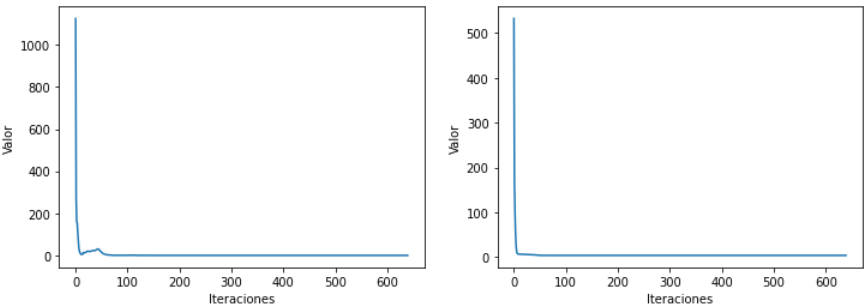
\includegraphics[scale=0.27]{1.png}}
    \caption{Gráficos de $||g_k||$ (izquierda) y $f(x_k)$ (derecha) a través de las iteraciones de la función de Rosembrock con GC-FR no lineal}
    \label{r1}
\end{figure}

\begin{figure}[htbp]
    \centerline{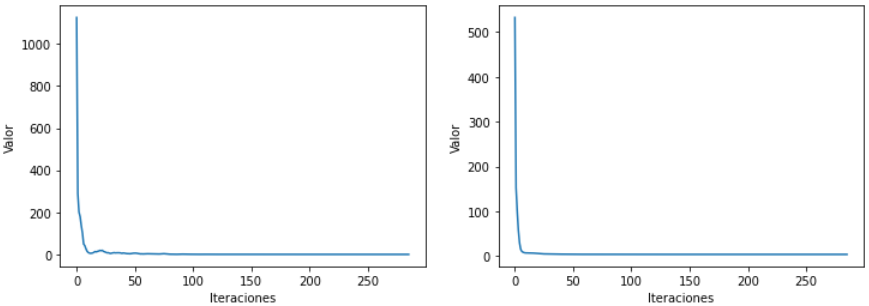
\includegraphics[scale=0.27]{2.png}}
    \caption{Gráficos de $||g_k||$ (izquierda) y $f(x_k)$ (derecha) a través de las iteraciones de la función de Rosembrock con GC-FRPR no lineal}
    \label{r2}
\end{figure}

\begin{figure}[htbp]
    \centerline{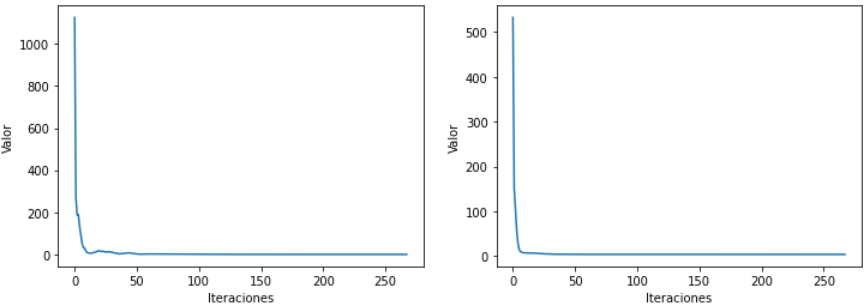
\includegraphics[scale=0.27]{3.png}}
    \caption{Gráficos de $||g_k||$ (izquierda) y $f(x_k)$ (derecha) a través de las iteraciones de la función de Rosembrock con GC-HS no lineal}
    \label{r3}
\end{figure}

\begin{figure}[htbp]
    \centerline{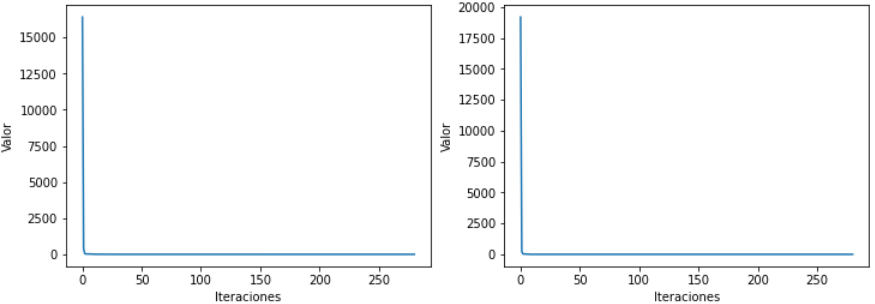
\includegraphics[scale=0.27]{4.png}}
    \caption{Gráficos de $||g_k||$ (izquierda) y $f(x_k)$ (derecha) a través de las iteraciones de la función de Wood con GC-FR no lineal}
    \label{r4}
\end{figure}

\begin{figure}[htbp]
    \centerline{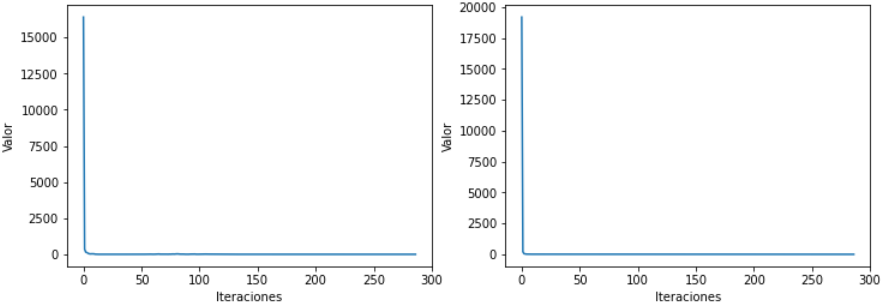
\includegraphics[scale=0.27]{5.png}}
    \caption{Gráficos de $||g_k||$ (izquierda) y $f(x_k)$ (derecha) a través de las iteraciones de la función de Wood con GC-FRPR no lineal}
    \label{r5}
\end{figure}

\begin{figure}[htbp]
    \centerline{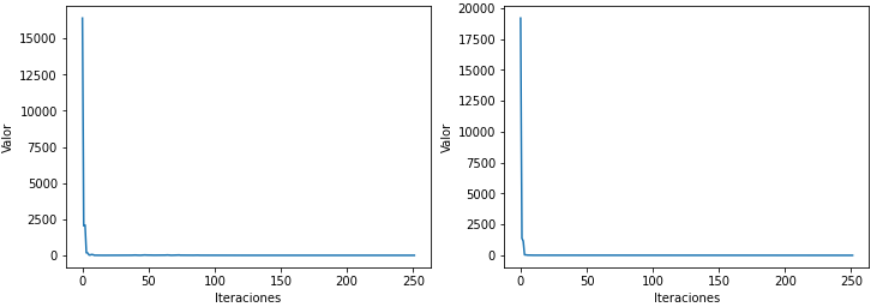
\includegraphics[scale=0.27]{6.png}}
    \caption{Gráficos de $||g_k||$ (izquierda) y $f(x_k)$ (derecha) a través de las iteraciones de la función de Wood con GC-HS no lineal}
    \label{r6}
\end{figure}

\section*{}

\begin{thebibliography}{00}
\bibitem{b1} Jorge Nocedal, Stephen J. Wright, ``Numerical Optimization,'' Second Edition, Springer.
\end{thebibliography}

\end{document}
